\documentclass[11pt,a4paper]{article}

% ---------------------------------------------------------------------------
% Zero-divisor methods for absolute concentration robustness:
% completeness, positive geometry, and quantitative certificates.
%
% Author metadata: fill in the three macros below before submission.
% ---------------------------------------------------------------------------
\newcommand{\PaperAuthor}{}
\newcommand{\PaperAffiliation}{}
\newcommand{\PaperDate}{20 September 2026}

\usepackage[T1]{fontenc}
\usepackage[utf8]{inputenc}
\usepackage{lmodern}
\usepackage{microtype}
\usepackage[a4paper,margin=1.05in]{geometry}
\usepackage{amsmath,amssymb,amsthm,mathtools}
\usepackage{booktabs}
\usepackage{array}
\usepackage{enumitem}
\usepackage{xcolor}
\usepackage{graphicx}
\usepackage{tikz}
\usetikzlibrary{arrows.meta,positioning,calc}
\usepackage[obeyspaces,spaces]{url}
\usepackage[numbers,sort&compress]{natbib}
\usepackage[colorlinks=true,linkcolor=blue!55!black,citecolor=blue!55!black,urlcolor=blue!55!black]{hyperref}
\hypersetup{pdftitle={Zero-divisor methods for absolute concentration robustness: completeness, positive geometry, and quantitative certificates},
  pdfsubject={Counterexamples, corrected Groebner-basis candidate coverage, regular-point geometry and quantitative certificates for absolute concentration robustness in mass-action systems},
  pdfkeywords={absolute concentration robustness, mass-action kinetics, steady-state ideal, zero divisor, Groebner basis, block order, regular local ring, certificate, EnvZ/OmpR, Lean}}

\DeclareUrlCommand\lean{\urlstyle{tt}}
\setlist{itemsep=2pt,topsep=3pt}
\setlength{\emergencystretch}{1.5em}

\theoremstyle{plain}
\newtheorem{theorem}{Theorem}[section]
\newtheorem{proposition}[theorem]{Proposition}
\newtheorem{lemma}[theorem]{Lemma}
\newtheorem{corollary}[theorem]{Corollary}
\theoremstyle{definition}
\newtheorem{definition}[theorem]{Definition}
\newtheorem{example}[theorem]{Example}
\theoremstyle{remark}
\newtheorem{remark}[theorem]{Remark}

\newcommand{\R}{\mathbb{R}}
\newcommand{\Q}{\mathbb{Q}}
\newcommand{\N}{\mathbb{N}}
\newcommand{\lc}{\operatorname{lc}}
\newcommand{\lmz}{\operatorname{lm}}
\newcommand{\LM}{\operatorname{LM}}
\newcommand{\rank}{\operatorname{rank}}
\newcommand{\tr}{\operatorname{tr}}
\newcommand{\muM}{\mu\mathrm{M}}
\newcommand{\permin}{\mathrm{min}^{-1}}
\newcommand{\Xtot}{X_{\mathrm{tot}}}
\newcommand{\Ytot}{Y_{\mathrm{tot}}}
\newcommand{\cin}{c_{\mathrm{in}}}

\title{Zero-divisor methods for absolute concentration robustness:\\[2pt]
\large completeness, positive geometry, and quantitative certificates}
\author{\PaperAuthor\\ \PaperAffiliation}
\date{\PaperDate}

\begin{document}
\maketitle

\begin{abstract}
A mass-action system has absolute concentration robustness (ACR) in a species whose concentration is the same at every positive steady state. Garc\'ia Puente, Gross, Harrington, Johnston, Meshkat, P\'erez Mill\'an and Shiu proposed to detect ACR values as the positive numbers $\alpha$ for which $x_i-\alpha$ lies in, or is a zero divisor of, the steady-state ideal, and to list them from the leading coefficients of a Gr\"obner basis. We settle two questions they left open. For networks with at most bimolecular complexes, uniqueness of such a value is neither necessary nor sufficient for ACR. Their candidate algorithm is incomplete for an elimination order that their definition admits, and we prove that it is complete for block orders, which establishes their conjecture in that form. We then show that one positive steady state at which the Jacobian has rank equal to the stoichiometric rank forces every ACR value, global or local, to be a zero-divisor value, with a multiplier that does not vanish at that state. The second half of the paper makes such identities quantitative: a lower bound on the multiplier converts a polynomial identity into a bound on $|x_i-\alpha|$ in terms of steady-state residuals and signed load terms, and without such a bound a small residual can indicate extinction instead of accuracy. For a loaded reactor we obtain the exact positive operating region, a strictly smaller conditioning region, local stability throughout, and an explicit rational Lyapunov ellipsoid on which the multiplier bound holds for all time. For the EnvZ/OmpR model every positive steady state is regular, steady states are classified by total amounts, and uniform multiplier bounds hold over parameter boxes. Finally, replacing a reaction that has more than two product molecules by a chain of private intermediates preserves the steady-state quotient ring, the positive steady states and all ACR values, while adding explicit residual, storage and leakage terms to a certificate. The algebraic results and the identities and inequalities behind the quantitative ones are compiled in Lean~4 with Mathlib; the geometric and dynamical arguments are conventional proofs and are marked as such.
\end{abstract}

\noindent\textbf{Keywords.} absolute concentration robustness; mass-action kinetics; steady-state ideal; zero divisor; Gr\"obner basis; block order; regular point; certificate; EnvZ/OmpR; formal verification.

\noindent\textbf{MSC 2020.} 92C42, 13P10, 13P25, 14P10, 37N25, 34D20.

\section{Introduction}\label{sec:intro}

\paragraph{Background.}
A biochemical network has \emph{absolute concentration robustness} (ACR) in a species $X_i$ if the concentration of $X_i$ is the same at every positive steady state, whatever the total amounts of the conserved moieties. The notion was introduced by Shinar and Feinberg \cite{shinarfeinberg}, who gave a deficiency-one structural criterion and used it to explain the experimentally observed insensitivity of the phosphorylated response regulator in the \emph{E.~coli} EnvZ/OmpR osmoregulation system to the amounts of its own signalling proteins \cite{batchelor,shinaralon}. Since then ACR has been studied through invariants and toric structure \cite{karp,toric}, in low-dimensional networks \cite{lowdim}, in local and generic forms \cite{localglobal,generic}, as a dynamical and control-theoretic property \cite{dynamic,integral}, and stochastically, where the same networks can reach extinction with probability one \cite{aej}.

For a fixed choice of rate constants ACR is a statement about the \emph{positive real} zeros of the steady-state polynomials, and deciding it is a problem of real algebraic geometry. Garc\'ia Puente, Gross, Harrington, Johnston, Meshkat, P\'erez Mill\'an and Shiu \cite{acr} analysed how far the steady-state \emph{ideal} can be used instead. They observed that in many examples the ACR value $\alpha$ is visible because $x_i-\alpha$ belongs to the ideal or is a zero divisor modulo it, called this \emph{zero-divisor ACR}, and asked the following.
\begin{itemize}
\item \emph{Question 3.13 of \cite{acr}.} Consider the condition that there is a \emph{unique} $\alpha>0$ such that $x_i-\alpha$ is in the steady-state ideal or is a zero divisor of it \cite[condition (13)]{acr}. It is neither necessary nor sufficient for ACR in general \cite[Examples 3.11 and 3.12]{acr}, but the known examples use complexes with three molecules. For networks that are at most bimolecular, is the condition necessary? Is it sufficient?
\item \emph{Conjecture 4.7 of \cite{acr}.} Algorithm~1 of \cite{acr} computes a reduced Gr\"obner basis for an elimination order and returns the positive roots of the univariate basis element or, when there is none, of the leading coefficients of the basis elements. The conjecture states that for rational rate constants every zero-divisor ACR value is returned.
\end{itemize}

\paragraph{Results.}
This paper answers both and then asks what is needed to turn such an algebraic candidate into a concentration guarantee that can be used on a specified domain.
\begin{enumerate}[label=(\arabic*)]
\item \emph{Question 3.13 has a negative answer in both directions} (Section~\ref{sec:counter}). A conservative five-reaction network has ACR in $A$ with value $2$ while $\{2,3\}$ are both zero-divisor values; the second value comes from a boundary component. A seven-reaction network has the single zero-divisor value $1$, supplied by an isolated point with a negative coordinate, and no ACR. All complexes in both networks have at most two molecules.
\item \emph{Conjecture 4.7 fails for the elimination orders admitted in \cite{acr} and holds for block orders} (Sections~\ref{sec:order} and~\ref{sec:block}). For a four-reaction network with ACR value $1$ we exhibit a monomial order that satisfies the definition of an elimination order in \cite{acr} but is not a block order; its reduced basis has leading coefficients $1,t,-1$ and no univariate element, so the algorithm returns nothing. For a block order we prove that multiplication by $t-a$ is injective modulo the ideal whenever $a$ is not a root of the product of the leading coefficients, over every field extension (Theorem~\ref{thm:block}). Completeness of the algorithm follows (Corollary~\ref{cor:complete}).
\item \emph{One regular positive steady state suffices for coverage} (Section~\ref{sec:geometry}). If the Jacobian of the mass-action field has rank equal to the stoichiometric rank at one positive steady state $x^*$, then every value that coordinate $i$ takes identically on the positive steady states near $x^*$ is a zero-divisor value, and the multiplier can be chosen nonzero at $x^*$ (Theorem~\ref{thm:regular}). In particular the corrected algorithm lists every ACR value, and an ACR value that it misses can occur only if \emph{every} positive steady state is rank deficient.
\item \emph{A multiplier floor turns an identity into an error bound} (Section~\ref{sec:bounds}). From $(x_i-\alpha)^m h=\sum_j q_jf_j$ and $|h|\ge h_0>0$ on a domain one obtains $|x_i-\alpha|\le((\sum_jQ_j\epsilon_j+\eta)/h_0)^{1/m}$ for residual bounds $\epsilon_j$ and a \emph{signed} load term $\eta$. Without the floor the statement is false: a small residual can indicate extinction of the multiplier instead of accuracy.
\item \emph{Worked systems.} A loaded reactor built from the first counterexample has an exact positive operating region, a strictly smaller region on which a prescribed floor holds, local asymptotic stability throughout, and an explicit forward-invariant ellipsoid with rational data (Section~\ref{sec:reactor}). For the EnvZ/OmpR model of \cite{shinarfeinberg} every positive steady state is regular, positive steady states are classified by the two total amounts, and uniform floors hold over parameter boxes (Section~\ref{sec:envz}).
\item \emph{Private product release} (Section~\ref{sec:release}). A reaction with more than two product molecules can be replaced by a chain of at-most-bimolecular steps through private intermediates without changing the steady-state quotient ring in the old coordinates, the positive steady states, or any zero-divisor or ACR value. Away from equilibrium the intermediates contribute explicit residual terms; at equilibrium they impose a storage cost inversely proportional to the release rates; leakage from them produces a computable certificate defect.
\end{enumerate}

Table~\ref{tab:map} summarises which question each result answers and what it leaves as an assumption.

\begin{table}[!htbp]
\centering\small
\begin{tabular}{@{}>{\raggedright\arraybackslash}p{0.29\textwidth}>{\raggedright\arraybackslash}p{0.30\textwidth}>{\raggedright\arraybackslash}p{0.34\textwidth}@{}}
\toprule
Question & Result & What remains an assumption\\
\midrule
Does bimolecularity make condition (13) of \cite{acr} characterise ACR? & No, in both directions (Props.~\ref{prop:necessity}, \ref{prop:sufficiency}) & ---\\
Does Algorithm~1 of \cite{acr} list every zero-divisor ACR value? & Not for every admitted order (Prop.~\ref{prop:order}); yes for block orders (Cor.~\ref{cor:complete}) & Exact root sets; a listed candidate need not be an ACR value\\
When is every ACR value a zero-divisor value? & When one positive steady state is regular (Thm.~\ref{thm:regular}) & Regularity is sufficient, not necessary\\
When does an identity bound $|x_i-\alpha|$? & When the multiplier has a floor on the domain (Thm.~\ref{thm:bound}) & The floor and the residual bounds on that domain\\
Where does the floor hold? & Equilibrium regions (Thms.~\ref{thm:reactor}, \ref{thm:envpool}); an invariant ellipsoid (Prop.~\ref{prop:ellipsoid}) & Entry into the region; fixed rates for the ellipsoid\\
What does bimolecular realisation cost? & Nothing at equilibrium (Thm.~\ref{thm:release}); residual, storage and leakage terms otherwise (Props.~\ref{prop:transport}--\ref{prop:leak}) & Existence of a leaking equilibrium in the domain\\
\bottomrule
\end{tabular}
\caption{The questions addressed and the scope of each answer.}\label{tab:map}
\end{table}

\paragraph{Relation to earlier work.}
The obstruction behind our second counterexample is the reduced algebra of \cite[Example 3.12]{acr}; what is new is a realisation with complexes of at most two molecules on both sides of every reaction, and a complete computation of the quotient. The EnvZ/OmpR topology and its ACR value are due to \cite{shinarfeinberg}, and the Gr\"obner basis we start from is displayed in \cite[Example 3.15]{acr}; our contribution there is the regularity certificate, the classification by totals and the floors. The idea behind Algorithm~1 of \cite{acr} comes from the stability of Gr\"obner bases under specialisation of parameters \cite{weispfenning,kalkbrener,suzuki,montes}. Theorem~\ref{thm:block} is proved directly by localisation and division by monic polynomials and does not rely on a specialisation theorem; Remark~\ref{rem:specialisation} records what our order example implies for the form of that theorem quoted in \cite{acr}. That a real prime ideal with a nonsingular real zero is real is classical \cite[Section~3.3]{bcr} and is recalled in \cite[Proposition 3.27]{acr}; their Theorem~3.28 uses it for a decomposition of an auxiliary positive-restriction ideal and a rational proposed value. Theorem~\ref{thm:regular} differs in using the original ideal, a single regular positive point, an arbitrary real value, and in producing a multiplier that is nonzero at the point. The generic-rate results of \cite[Theorem~4.4 and Corollary~4.7]{generic} characterise ACR for almost all rate constants and concern a different quantifier. Elimination of intermediates at steady state is well developed \cite{fwlinear,fwptm,fwintermediate}; Section~\ref{sec:release} treats a triangular special case in which an intermediate appears in a product complex together with a released species, which is outside the definition of intermediates in \cite{fwintermediate}, and adds the non-equilibrium bookkeeping. The distinction between static and dynamic ACR \cite{dynamic}, the integral-feedback structure of ACR systems \cite{integral} and stochastic extinction \cite{aej} are the natural context for the multiplier floors of Sections~\ref{sec:bounds}--\ref{sec:envz}.

\paragraph{Evidence.}
The counterexamples, the completeness theorem for block orders, the release algebra and the polynomial identities and inequalities of Sections~\ref{sec:bounds}--\ref{sec:release} are compiled in Lean~4 \cite{lean4} with Mathlib \cite{mathlib}. The regular-point geometry, the passage from the spectrum to nonlinear stability, the invariance argument and the existence parts of the pool classification are conventional proofs given here in full. Section~\ref{sec:formal} states the boundary result by result. All numerical statements about parameter boxes are exact rational enclosures; floating-point numbers appear only in figures.

\section{Setting and conventions}\label{sec:setting}

\paragraph{Mass action.}
A network has species $X_1,\dots,X_n$ and reactions $y_r\to y_r'$, $r=1,\dots,m$, with $y_r,y_r'\in\N^n$ and rate constants $\kappa_r>0$. The deterministic mass-action field is
\begin{equation}\label{eq:massaction}
  f(x)=\sum_{r=1}^m\kappa_r\,x^{y_r}\,(y_r'-y_r)=\Gamma\,v(x),
\end{equation}
where $\Gamma\in\mathbb{Z}^{n\times m}$ has columns $y_r'-y_r$ and $v_r(x)=\kappa_rx^{y_r}$. We write $n$ for the number of species and $s=\rank\Gamma$ for the \emph{stoichiometric rank}. A reaction $2B\to\varnothing$ with rate constant $\kappa$ has flux $\kappa b^2$ and contributes $-2\kappa b^2$ to $\dot b$; no stochastic factorial convention is used. A network is \emph{two-sided bimolecular} if $|y_r|\le2$ and $|y_r'|\le2$ for every reaction, where $|y|=\sum_iy_i$. This is the ``at most bimolecular'' condition of \cite{acr}.

\paragraph{The ideal.}
For a field $K$ containing the rate constants, $I_K=\langle f_1,\dots,f_n\rangle\subset K[x_1,\dots,x_n]$ is the \emph{steady-state ideal}. For rational rate constants we distinguish $I_\Q$ from its extension $I_\R=I_\Q\,\R[x]$. Throughout, $I$ is this original ideal. It is never replaced by its radical, by a saturation, by an ideal that includes conservation relations, or by the positive-restriction ideal of \cite{acr}; each of those changes the question.

\paragraph{Three sets.}
Let $V_+(I)=\{x\in\R^n_{>0}:f(x)=0\}$. Coordinate $i$ has (\emph{nonvacuous}) ACR with value $a$ if $V_+(I)\ne\varnothing$ and $x_i=a$ for every $x\in V_+(I)$. For a fixed coordinate $i$ we write
\begin{align*}
  P_i&=\{a>0:\ V_+(I)\neq\varnothing\text{ and }x_i=a\text{ on }V_+(I)\},\\
  Z_i&=\{a>0:\ x_i-a\in I_\R,\ \text{or there is }h\notin I_\R\text{ with }(x_i-a)h\in I_\R\},
\end{align*}
and $C_i$ for the set of positive real numbers returned by the candidate algorithm for a stated basis and order. Thus $P_i$ has at most one element, condition~(13) of \cite{acr} says that $Z_i$ is a singleton, and \emph{zero-divisor ACR} with value $a$ \cite[Definition 4.2]{acr} means $a\in P_i\cap Z_i$. Including ideal membership in $Z_i$ avoids a convention on whether the zero class is called a zero divisor; in all our examples the class of $x_i-a$ is nonzero.

\paragraph{Orders and the algorithm.}
Fix $i$, write $t=x_i$ and $z$ for the remaining variables. In \cite[Section~4.1]{acr} an \emph{elimination order} for $z$ is a monomial order on $K[t,z]$ such that every polynomial whose leading monomial lies in $K[t]$ itself lies in $K[t]$; equivalently, every monomial that involves some $z$-variable exceeds every power of $t$. A \emph{block order} (product order) first compares the $z$-parts of two monomials in a fixed monomial order $\succ_z$ and breaks ties by the exponent of $t$. Every block order is an elimination order, and \cite{acr} lists lexicographic and product orders as examples, but the definition admits more. For an elimination order, $\lc_z(g)\in K[t]$ denotes the coefficient of the $\succ_z$-largest $z$-monomial of $g$ regarded as a polynomial in $z$ over $K[t]$, where $\succ_z$ is the restriction of the order to monomials in $z$.

Algorithm~1 of \cite{acr}, for rational rate constants and each $i$, computes a reduced Gr\"obner basis $G$ of $I_\Q$ for an elimination order for $z$. If $G\cap\Q[t]\neq\varnothing$ it returns the positive roots of the unique element of $G\cap\Q[t]$. Otherwise it returns the positive roots of $\lc_z(g)$ for all $g\in G$. We regard the output $C_i$ as an exact set of real algebraic numbers; isolating roots numerically is a separate matter.

\section{Bimolecular counterexamples to condition (13)}\label{sec:counter}

\subsection{Necessity fails: a boundary component adds a value}

Consider five reactions with the indicated rate constants:
\begin{equation}\label{eq:necnet}
A+B\xrightarrow{1}2B,\qquad B\xrightarrow{1}A,\qquad B\xrightarrow{1}C,\qquad A+C\xrightarrow{1}2C,\qquad C\xrightarrow{3}A.
\end{equation}
With concentrations $(a,b,c)$ the field is
\begin{equation}\label{eq:necfield}
\dot a=-ab+b-ac+3c,\qquad \dot b=b(a-2),\qquad \dot c=c(a-3)+b.
\end{equation}
Every complex has at most two molecules, and $a+b+c$ is conserved.

\begin{proposition}\label{prop:necessity}
For the network \eqref{eq:necnet}, $V_+(I)=\{(2,\tau,\tau):\tau>0\}$, so $P_A=\{2\}$, while $Z_A=\{2,3\}$. Hence $A$ has ACR and condition~(13) of \cite{acr} fails.
\end{proposition}
\begin{proof}
At a positive steady state $\dot b=0$ forces $a=2$ and then $\dot c=0$ forces $b=c$; conversely $(2,\tau,\tau)$ is a steady state. This gives $V_+(I)$ and $P_A$.

Since $\dot a=-(\dot b+\dot c)$, the ideal is $I=\langle b(a-2),\,c(a-3)+b\rangle$. The second generator is monic and linear in $b$, so substituting $b=-c(a-3)$ gives an isomorphism
\[
  \R[a,b,c]/I\;\cong\;\R[a,c]/\bigl(c(a-2)(a-3)\bigr)
\]
that fixes $a$ and $c$. In the unique factorisation domain $\R[a,c]$, if $\gamma\notin\{2,3\}$ then $a-\gamma$ is coprime to $c(a-2)(a-3)$, so $(a-\gamma)h\in(c(a-2)(a-3))$ implies $h\in(c(a-2)(a-3))$, and $\gamma\notin Z_A$. For $\gamma\in\{2,3\}$ the complementary factor is a nonzero annihilator of $a-\gamma$ and $a-\gamma$ is not in the ideal. Explicitly, in the original ring,
\[
 (a-2)\,b\in I,\qquad (a-3)\,c(a-2)=(a-2)\bigl(c(a-3)+b\bigr)-b(a-2)\in I,
\]
while $b\notin I$ and $c(a-2)\notin I$ because they take the value $1$ at the zeros $(2,1,1)$ and $(3,0,1)$ of $I$, respectively.
\end{proof}

\begin{figure}[ht]
\centering
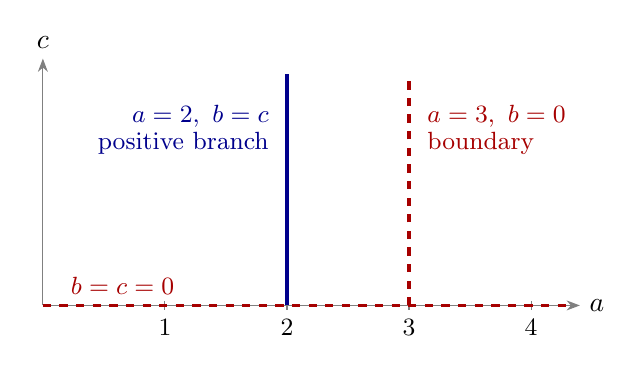
\begin{tikzpicture}[x=1.55cm,y=0.95cm,>=Stealth]
  \draw[->,gray] (0,0)--(4.4,0) node[right,black]{$a$};
  \draw[->,gray] (0,0)--(0,3.3) node[above,black]{$c$};
  \foreach \x in {1,2,3,4} \draw[gray] (\x,0.06)--(\x,-0.06) node[below,black]{\small$\x$};
  \draw[line width=1.3pt,blue!55!black] (2,0)--(2,3.1);
  \draw[line width=1.3pt,red!65!black,dashed] (3,0)--(3,3.1);
  \draw[line width=1.3pt,red!65!black,dashed] (0,0)--(4.3,0);
  \node[blue!55!black,anchor=east,align=right] at (1.93,2.35) {\small $a=2,\ b=c$\\[-2pt]\small positive branch};
  \node[red!65!black,anchor=west,align=left] at (3.07,2.35) {\small $a=3,\ b=0$\\[-2pt]\small boundary};
  \node[red!65!black,anchor=south west] at (0.15,0.02) {\small $b=c=0$};
\end{tikzpicture}
\caption{The real zero set of the steady-state ideal of \eqref{eq:necnet}, projected to the $(a,c)$-plane; $b=-c(a-3)$ on it. Only the component $a=2$ meets the positive orthant. The component $a=3$ lies in the boundary face $b=0$ and contributes the second zero-divisor value.}\label{fig:necessity}
\end{figure}

The algebra is correct and the value $3$ is excluded only by strict positivity (Figure~\ref{fig:necessity}). In the class $a+b+c=M$ with $M>2$ the unique positive steady state is $(2,(M-2)/2,(M-2)/2)$; as $M\downarrow2$ it approaches the boundary and the multiplier $b$ of the identity $(a-2)b=\dot b$ tends to zero. The same geometry therefore reappears as a conditioning problem in Section~\ref{sec:reactor}.

\subsection{Sufficiency fails: a nonpositive point supplies the only value}

Consider four species and seven reactions:
\begin{equation}\label{eq:sufnet}
\begin{gathered}
2A\xrightarrow{1}A+C,\qquad C\xrightarrow{1}A+D,\qquad D\xrightarrow{1}A+B,\qquad A+B\xrightarrow{1}B,\\
B\xrightarrow{1}A+B,\qquad A\xrightarrow{1}\varnothing,\qquad 2B\xrightarrow{1/2}\varnothing.
\end{gathered}
\end{equation}
The field is
\begin{equation}\label{eq:suffield}
f_A=-a^2+c+d-ab+b-a,\qquad f_B=d-b^2,\qquad f_C=a^2-c,\qquad f_D=c-d.
\end{equation}

\begin{proposition}\label{prop:sufficiency}
The network \eqref{eq:sufnet} is two-sided bimolecular, $V_+(I)=\{(\tau,\tau,\tau^2,\tau^2):\tau>0\}$, so $A$ does not have ACR, and $Z_A=\{1\}$. Hence condition~(13) of \cite{acr} holds and ACR fails.
\end{proposition}
\begin{proof}
One has the identities
\begin{equation}\label{eq:sufid}
  f_A+2f_C+f_D=(a-1)(a-b),\qquad f_B+f_C+f_D=(a-b)(a+b).
\end{equation}
The generators $f_C,f_D$ are monic and linear in $c$ and $d$; substituting $c=d=a^2$ and using \eqref{eq:sufid} gives $\R[a,b,c,d]/I\cong\R[a,b]/J$ with $J=(a-b)\,\mathfrak p$, $\mathfrak p=\langle a-1,a+b\rangle=\langle a-1,b+1\rangle$, by an isomorphism fixing $a$ and $b$. Since $(a-b)-2(a-1)+(a+b)=2$, the ideals $(a-b)$ and $\mathfrak p$ are comaximal, so their product is their intersection and the Chinese remainder theorem gives
\[
  \R[a,b]/J\;\cong\;\R[a,b]/(a-b)\times\R[a,b]/\mathfrak p\;\cong\;\R[a]\times\R,\qquad a\longmapsto(a,1).
\]
The image of $a-\gamma$ is $(a-\gamma,\,1-\gamma)$. In $\R[a]\times\R$ an element is a zero divisor exactly when one of its components is zero, because $\R[a]$ is a domain. The first component is never zero and the second is zero only for $\gamma=1$. Hence $Z_A=\{1\}$; an explicit witness is $(a-1)(a-b)\in I$ with $a-b\notin I$, since $a-b=2$ at the zero $(1,-1,1,1)$ of $I$.

At a positive steady state $c=d=a^2$ and $(a-b)(a+b)=0$ with $a+b>0$ give $a=b$; conversely the displayed points are steady states. The points with $\tau=1$ and $\tau=2$ show that $A$ is not ACR.
\end{proof}

The value $1$ is supplied by the isolated real point $(a,b)=(1,-1)$, which is a separate reduced component and not an embedded prime, while the positive diagonal admits every $a>0$. The reduced algebra $\dot a=(a-1)(a-b)$, $\dot b=(a-b)(a+b)$ is that of \cite[Example 3.12]{acr}, where it is realised with the complex $3A+B$; the network \eqref{eq:sufnet} realises an ideal with the same quotient using complexes of at most two molecules. We do not claim that either counterexample is minimal in the number of species or reactions.

\section{An admissible elimination order that misses the ACR value}\label{sec:order}

Take three species $T,U,V$ and the four reactions, all with rate constant $1$,
\begin{equation}\label{eq:ordernet}
T+U\to T,\qquad V\to U+V,\qquad U\to U+V,\qquad T+V\to T .
\end{equation}
The field is $\dot t=0$, $\dot u=v-tu$, $\dot v=u-tv$, and $I=\langle tu-v,\ tv-u\rangle$. At a positive steady state $u=tv=t^2u$ gives $t=1$ and $u=v$, and $(1,\tau,\tau)$ is a steady state for every $\tau>0$. So $T$ has ACR with value $1$. Moreover
\[
  (t-1)(u+v)=(tu-v)+(tv-u)\in I ,
\]
while $u+v\notin I$ (it equals $2$ at the zero $(1,1,1)$) and $t-1\notin I$ (it equals $-1$ at the zero $(0,0,0)$). Thus $1\in P_T\cap Z_T$: this is zero-divisor ACR.

Order the monomials $u^iv^jt^k$ by comparing the keys
\begin{equation}\label{eq:key}
  (\,i+j,\ k,\ i\,)\in\N^3
\end{equation}
lexicographically. The key is additive in the exponent vector and injective ($j$ is recovered from the first and third entries), so this is a total order compatible with multiplication, with $1$ as least element; it is a monomial order. Every monomial with $i+j>0$ exceeds every power of $t$, so it is an elimination order for $(u,v)$ in the sense of \cite{acr}. It is not a block order: among monomials of equal $(u,v)$-degree the exponent of $t$ is compared before the exponent of $u$, so for instance $vt\succ u$ although $u\succ_z v$ in the restricted order.

\begin{proposition}\label{prop:order}
For the order \eqref{eq:key} the reduced Gr\"obner basis of $I_\Q$ is
\[
  G=\{\,u^2-v^2,\ \ ut-v,\ \ vt-u\,\}.
\]
It has no element in $\Q[t]$, and $\lc_z$ of its elements are $1$, $t$ and $-1$. Algorithm~1 of \cite{acr} therefore returns no candidate for $T$, although $T$ has zero-divisor ACR with value $1$.
\end{proposition}
\begin{proof}
First, $u^2-v^2=v(ut-v)-u(vt-u)\in I$. The leading monomials for \eqref{eq:key} are $u^2$ (keys $(2,0,2)>(2,0,0)$), $ut$ (keys $(1,1,1)>(1,0,0)$) and $vt$ (keys $(1,1,0)>(1,0,1)$). Call a monomial \emph{standard} if it is divisible by none of $u^2,ut,vt$; the standard monomials are the powers $t^k$ and the monomials $u^\epsilon v^{d-\epsilon}$ with $d\ge1$ and $\epsilon\in\{0,1\}$.

Define a $\Q$-linear map $N$ on $\Q[u,v,t]$ on monomials by $N(t^k)=t^k$ and, for $d=i+j>0$,
\[
  N(u^iv^jt^k)=u^{\epsilon}v^{d-\epsilon},\qquad \epsilon=(i+k)\bmod 2 .
\]
For every monomial $\mu=u^iv^jt^k$ one checks $N(\mu\cdot ut)=N(\mu\cdot v)$ and $N(\mu\cdot vt)=N(\mu\cdot u)$: in each pair the total $(u,v)$-degree is $d+1$ and the parity of the $u$-exponent plus the $t$-exponent agrees. Hence $N$ vanishes on $I$. Moreover $N$ fixes standard monomials, and $N(\mu)\prec\mu$ for every nonstandard $\mu$: if $k>0$ the second key entry drops to $0$, and if $k=0$ then $i\ge2$ and the third entry drops. Now let $0\neq p\in I$ and suppose $\LM(p)$ were standard. Then $N(p)=0$, but $N$ fixes $\LM(p)$ and sends every other monomial of $p$ to a monomial at most itself, hence smaller than $\LM(p)$; so the coefficient of $\LM(p)$ in $N(p)$ is nonzero, a contradiction. Thus every leading monomial of $I$ is divisible by $u^2$, $ut$ or $vt$, and $G$ is a Gr\"obner basis. It is reduced: the elements are monic, no leading monomial divides another, and the tails $v^2,v,u$ are standard.

The restriction of \eqref{eq:key} to monomials in $u,v$ compares total degree and then the exponent of $u$. As polynomials in $u,v$ over $\Q[t]$ the three basis elements have leading terms $1\cdot u^2$, $t\cdot u$ and $-1\cdot u$. No leading coefficient has a positive root and $G\cap\Q[t]=\varnothing$, so the output is empty.
\end{proof}

For comparison, the lexicographic order $u\succ v\succ t$, which is a block order, has reduced basis $\{u-tv,\ (t^2-1)v\}$ and the algorithm returns the candidate $1$. The example refutes Conjecture~4.7 of \cite{acr} only under the unrestricted reading of ``an elimination order'', which is the reading that the definition and Algorithm~1 there allow; it does not affect lexicographic or product orders, for which the conjecture is proved in the next section. The mechanism is that, for an elimination order that is not a block order, the $z$-part of the leading monomial of $g$ need not be the $\succ_z$-leading $z$-monomial of $g$: for $vt-u$ these are $v$ and $u$.

\begin{remark}[Specialisation]\label{rem:specialisation}
Lemma~4.14 of \cite{acr}, a rephrasing of a result of Suzuki and Sato \cite{suzuki} which motivated Algorithm~1, states that for a reduced Gr\"obner basis $G$ for an elimination order and any $\alpha$ at which no $\lc_z(g)$, $g\in G\setminus\Q[t]$, vanishes, the specialised set $G|_{t=\alpha}$ is a reduced Gr\"obner basis of $I|_{t=\alpha}$ for $\succ_z$. For the order \eqref{eq:key} this also requires the block hypothesis. At $\alpha=2$ the leading coefficients $1,2,-1$ are nonzero, the specialised ideal $\langle 2u-v,2v-u\rangle$ equals $\langle u,v\rangle$, and it contains $v$, whose leading monomial is not divisible by the leading monomials $u^2,u,u$ of $G|_{t=2}$. We make no statement about the hypotheses of the original result in \cite{suzuki}; stability under specialisation is classically formulated for block orders \cite{kalkbrener,montes}.
\end{remark}

\section{Completeness for block orders}\label{sec:block}

Let $K$ be a field, $t$ a single variable and $z=(z_1,\dots,z_N)$. Fix a monomial order $\succ_z$ on the monomials in $z$ and let $\succ$ be the block order on $K[t,z]$ that compares $z$-parts by $\succ_z$ and breaks ties by the exponent of $t$. For $0\neq g\in K[t][z]$ write $\lmz_z(g)$ for its $\succ_z$-largest $z$-monomial and $\lc_z(g)\in K[t]\setminus\{0\}$ for its coefficient. For a block order,
\begin{equation}\label{eq:blockprop}
  \LM(g)=\lmz_z(g)\cdot t^{\deg\lc_z(g)} .
\end{equation}
Let $G=\{g_1,\dots,g_r\}$ be a Gr\"obner basis, with nonzero elements, of a proper ideal $I\subset K[t,z]$ for $\succ$, and put
\[
  H(t)=\prod_{j=1}^r\lc_z(g_j)\in K[t]\setminus\{0\}.
\]
For an element $g_j\in K[t]$ one has $\lc_z(g_j)=g_j$. For a field extension $L/K$ write $I_L=I\,L[t,z]$.

\begin{theorem}[Coefficient exceptional set]\label{thm:block}
Let $L/K$ be a field extension and $a\in L$ with $H(a)\neq0$. Then multiplication by $t-a$ is injective on $L[t,z]/I_L$. If in addition $I\cap K[t]=0$, then $t-a\notin I_L$.
\end{theorem}
\begin{proof}
\emph{Step 1: $G$ is a Gr\"obner basis of $I_L$.} Let $0\neq p\in I_L$ with leading coefficient $c\in L$. Choose a $K$-linear functional $\phi\colon L\to K$ with $\phi(c)\neq0$ and apply it coefficientwise to obtain $\phi_*\colon L[t,z]\to K[t,z]$. This map is $K[t,z]$-linear, so writing $p=\sum_ja_jg_j$ with $a_j\in L[t,z]$ gives $\phi_*(p)=\sum_j\phi_*(a_j)g_j\in I$. The support of $\phi_*(p)$ is contained in that of $p$ and contains $\LM(p)$, so $\LM(\phi_*(p))=\LM(p)$ and some $\LM(g_j)$ divides it. The same argument applied to a nonzero element of $I_L\cap L[t]$ shows that $I\cap K[t]=0$ implies $I_L\cap L[t]=0$.

\emph{Step 2: localisation.} Put $D=L[t,H^{-1}]$, a domain, and $I_D=I_L\,D[z]$. Each $\lc_z(g_j)$ divides $H$ and is a unit of $D$, so after scaling each $g_j$ is monic in $D[z]$ with respect to $\succ_z$. We claim that for every nonzero $p\in I_D$ some $\lmz_z(g_j)$ divides $\lmz_z(p)$. Indeed $H^Mp=q$ for some $M$ and some $q\in I_L$; multiplication by the nonzero element $H^M$ of the domain $D$ does not change the $z$-support, so $\lmz_z(p)=\lmz_z(q)$. By Step~1 some $\LM(g_j)$ divides $\LM(q)$, and by \eqref{eq:blockprop} their $z$-parts are $\lmz_z(g_j)$ and $\lmz_z(q)$. This is the only place where the block hypothesis is used.

\emph{Step 3: division.} Division by the monic polynomials $g_j$ in $D[z]$ writes any $h\in D[z]$ as $h=\sum_jb_jg_j+\rho$, where no $z$-monomial of $\rho$ is divisible by any $\lmz_z(g_j)$. Suppose $(t-a)h\in I_L$ with $h\in L[t,z]$. Then $(t-a)\rho\in I_D$. If $\rho\neq0$, then $(t-a)\rho\neq0$ because $D$ is a domain and $t-a\neq0$ in it, and $\lmz_z((t-a)\rho)=\lmz_z(\rho)$ is divisible by no $\lmz_z(g_j)$, contradicting Step~2. Hence $\rho=0$, so $h\in I_D$ and $H^Mh\in I_L$ for some $M\ge0$.

\emph{Step 4: removing the denominator.} Division in $L[t]$ gives $H^M=(t-a)Q+H(a)^M$. Then $H(a)^Mh=H^Mh-Q\,(t-a)h\in I_L$, and $H(a)^M$ is a nonzero element of $L$, so $h\in I_L$. This proves injectivity. Finally, if $I\cap K[t]=0$ then $I_L\cap L[t]=0$ by Step~1, so $t-a\notin I_L$.
\end{proof}

Step~3 also shows that the standard $z$-monomials form a basis of $D[z]/I_D$ as a free $D$-module, possibly of infinite rank. One must not localise further to $L(t)$: that would make $t-a$ invertible and erase the torsion that is being located.

\begin{corollary}[Completeness of the candidate algorithm for block orders]\label{cor:complete}
Let the rate constants be rational, fix a coordinate $t=x_i$, and let $G$ be a Gr\"obner basis of $I_\Q$ for a block order in which the remaining variables are compared first. If $V_+(I)\neq\varnothing$ and $\alpha\in P_i\cap Z_i$, then $\alpha$ is returned by Algorithm~1 of \cite{acr}. More precisely:
\begin{enumerate}[label=(\alph*)]
\item if $G$ contains a univariate element $\tilde h\in\Q[t]$, then $\tilde h(\alpha)=0$ for every $\alpha\in P_i$, for any elimination order;
\item if $G\cap\Q[t]=\varnothing$, then every $\alpha\in Z_i$ is a root of $\lc_z(g)$ for some $g\in G$; the same holds for every element $\alpha$ of an extension field $L$ of $\Q$ such that $t-\alpha$ lies in $I_L$ or is a zero divisor modulo $I_L$.
\end{enumerate}
In particular Conjecture~4.7 of \cite{acr} holds for block orders.
\end{corollary}
\begin{proof}
(a) A positive steady state $x$ has $x_i=\alpha$ and is a zero of $\tilde h\in I$. (b) By the elimination theorem \cite[Chapter~3]{clo}, $I_\Q\cap\Q[t]=0$. If $\alpha\in Z_i$, then either $t-\alpha\in I_\R$, which Theorem~\ref{thm:block} excludes when $H(\alpha)\neq0$, or $(t-\alpha)h\in I_\R$ with $h\notin I_\R$, which contradicts injectivity when $H(\alpha)\neq0$. So $H(\alpha)=0$, and a product in a field vanishes only if a factor does.
\end{proof}

The corollary neither asserts that a returned candidate is an ACR value (Proposition~\ref{prop:necessity} returns $\{2,3\}$) nor that every system with ACR has a zero-divisor value (see \cite[Example 3.11]{acr} and Section~\ref{sec:geometry}), and it carries no complexity bound.

\section{Coverage from one regular positive steady state}\label{sec:geometry}

Theorem~\ref{thm:block} covers values in $Z_i$. We now give a geometric condition under which every ACR value lies in $Z_i$. Recall from \eqref{eq:massaction} that $f=\Gamma v$ with $\rank\Gamma=s$. Choose $s$ linearly independent rows of $\Gamma$ and let $\psi=(\psi_1,\dots,\psi_s)$ be the corresponding coordinates of $f$. Every $f_j$ is a constant linear combination of $\psi_1,\dots,\psi_s$, so
\begin{equation}\label{eq:psi}
  I=\langle\psi_1,\dots,\psi_s\rangle,\qquad \rank Df(x)=\rank D\psi(x)\le s\quad\text{for all }x .
\end{equation}

\begin{definition}\label{def:regular}
A positive steady state $x^*$ is \emph{regular} if $\rank Df(x^*)=s$, the stoichiometric rank.
\end{definition}

\begin{theorem}[Regular-point coverage]\label{thm:regular}
Let $x^*\in V_+(I)$ be regular, and suppose that for some neighbourhood $U$ of $x^*$ and some $\alpha\in\R$ one has $x_i=\alpha$ for all $x\in V_+(I)\cap U$. Then there is a polynomial $h\in\R[x]$ with
\begin{equation}\label{eq:regularwitness}
  (x_i-\alpha)\,h\in I_\R\qquad\text{and}\qquad h(x^*)\neq0 .
\end{equation}
In particular $h\notin I_\R$ and $\alpha\in Z_i$. Consequently, if the system has a regular positive steady state, then $P_i\subset Z_i$, and for rational rate constants the candidate set $C_i$ of a block order contains every ACR value of coordinate $i$.
\end{theorem}
\begin{proof}
All ideals are in $\R[x]$. Let $\mathfrak m$ be the maximal ideal of $x^*$, $\mathcal O=\R[x]_{\mathfrak m}$, and $A=\mathcal O/I\mathcal O$.

\emph{Step 1: $A$ is a regular local ring, hence a domain.} The ring $\mathcal O$ is regular local of dimension $n$ with residue field $\R$, and $\mathfrak m\mathcal O/\mathfrak m^2\mathcal O\cong\R^n$ by $p\mapsto\nabla p(x^*)$. The images of $\psi_1,\dots,\psi_s\in\mathfrak m$ are the rows of $D\psi(x^*)$, which are linearly independent by regularity and \eqref{eq:psi}. Hence $\psi_1,\dots,\psi_s$ is part of a regular system of parameters and $A=\mathcal O/(\psi)$ is regular local of dimension $n-s$ \cite[Theorem~14.2]{matsumura}; a regular local ring is a domain \cite[Theorem~14.3]{matsumura}. Therefore
\[
  P:=I\mathcal O\cap\R[x]=\{p\in\R[x]:\ wp\in I\text{ for some }w\notin\mathfrak m\}
\]
is a prime ideal with $I\subset P\subset\mathfrak m$. Let $p_1,\dots,p_\ell$ generate $P$ and choose $w_l\notin\mathfrak m$ with $w_lp_l\in I$. Then $h:=w_1\cdots w_\ell$ satisfies
\begin{equation}\label{eq:hP}
  h\,P\subset I,\qquad h(x^*)\neq0 .
\end{equation}

\emph{Step 2: $x_i-\alpha\in P$.} After reordering coordinates write $x=(x',x'')$ with $x''\in\R^s$ and $\partial\psi/\partial x''(x^*)$ invertible. By the real-analytic implicit function theorem there are a neighbourhood $U'\subset U$ of $x^*$, a neighbourhood $W$ of $(x^*)'$ and a real-analytic map $\varphi\colon W\to\R^s$ with
\[
  \{x\in U':\psi(x)=0\}=\{(x',\varphi(x')):x'\in W\}.
\]
Shrinking $W$, all these points are positive, hence lie in $V_+(I)\cap U$, and so the analytic function $x'\mapsto p(x',\varphi(x'))$ with $p=x_i-\alpha$ vanishes identically on $W$.

Let $\widehat{\mathcal O}=\R[[x-x^*]]$ be the completion of $\mathcal O$. The formal implicit function theorem gives a unique $\widehat\varphi\in\R[[x'-(x^*)']]^s$ with $\widehat\varphi(0)=(x^*)''$ and $\psi(x',\widehat\varphi)=0$, and by uniqueness $\widehat\varphi$ is the Taylor series of $\varphi$. In the coordinates $(x',y)$ with $y=x''-\widehat\varphi(x')$ one has $\psi=M\,y$ for a matrix $M$ of power series with $M(0)=\partial\psi/\partial x''(x^*)$ invertible, so $(\psi)\widehat{\mathcal O}=(y)\widehat{\mathcal O}$ and
\[
  \widehat A=\widehat{\mathcal O}/(\psi)\;\cong\;\R[[x'-(x^*)']],\qquad x''\longmapsto\widehat\varphi(x') .
\]
Under the composite $\R[x]\to A\to\widehat A$ the polynomial $p$ maps to the Taylor series of $p(x',\varphi(x'))$ at $(x^*)'$, which is zero. Since $A$ is a Noetherian local ring, $A\to\widehat A$ is injective by Krull's intersection theorem \cite[Theorem~8.10]{matsumura}. Hence $p\in I\mathcal O\cap\R[x]=P$.

\emph{Step 3.} By \eqref{eq:hP}, $(x_i-\alpha)h\in I$ and $h(x^*)\neq0$; since every element of $I$ vanishes at $x^*$, $h\notin I$. The remaining statements follow from the definitions and Corollary~\ref{cor:complete}, the positive point $x^*$ providing nonvacuity.
\end{proof}

\begin{remark}\label{rem:minimalprime}
The prime $P$ of the proof is the unique minimal prime of $I$ contained in $\mathfrak m$, because primes of $\R[x]$ between $I$ and $\mathfrak m$ correspond to primes of the domain $A$. It is therefore an associated prime of $I$ \cite[Theorem~6.5]{matsumura}, and the statement $\alpha\in Z_i$ could also be derived from that fact. The direct construction \eqref{eq:hP} gives more: the multiplier is nonzero at $x^*$, so by continuity $|h|\ge h_0>0$ on a neighbourhood of $x^*$, which is exactly the hypothesis of the quantitative Theorem~\ref{thm:bound} with $m=1$. In this sense a regular positive steady state is always locally well conditioned, although the theorem does not provide $h$ or the neighbourhood explicitly. Since only $x_i=\alpha$ near $x^*$ is used, the theorem also applies to the values of \emph{local} ACR in the sense of \cite{localglobal}.
\end{remark}

\begin{corollary}\label{cor:missed}
Suppose the rate constants are rational and the system has a regular positive steady state. If the candidate set of a block order for coordinate $i$ is empty, then coordinate $i$ does not have ACR. An ACR value that is missed by the corrected algorithm can occur only if $\rank Df(x)<s$ at every positive steady state $x$.
\end{corollary}

The hypothesis is sufficient, not necessary, and one regular point is enough. It does not infer ACR from a unique candidate. It is weaker than nondegeneracy in a stoichiometric compatibility class, which asks that $Df(x^*)$ be injective on the stoichiometric subspace; appending conservation equations to isolate a steady state does not by itself verify it. If $s=0$ the field vanishes identically and no coordinate has ACR.

\begin{remark}[What regularity is not]\label{rem:notdeficiency}
We have no estimate of how often regularity fails in models of practical interest, and the following distinctions should be kept. The deficiency of a network is a combinatorial invariant and does not force $\rank Df<s$. Multistationarity is compatible with regularity at every positive steady state. A saddle-node within a compatibility class need not be rank deficient in our sense: the steady-state set can be a smooth manifold of dimension $n-s$ on which the map to the conserved totals has a critical point. Rank deficiency can be structural, can occur for special rate constants, or can reflect singular positive geometry; testing the $s\times s$ minors of $D\psi$ on $V_+(I)$ identifies which. A nonzero minor at a point that is not a steady state certifies nothing. For generic rate constants the relevant nondegeneracy theory is developed in \cite{generic}.
\end{remark}

\begin{example}[The examples of this paper]\label{ex:ranks}
For \eqref{eq:necnet}, $s=2$, $\psi=(b(a-2),\,c(a-3)+b)$, and the $(a,b)$-minor of $D\psi$ at $(2,1,1)$ equals $1$; the witness $h=b$ is nonzero there. For \eqref{eq:ordernet}, $s=2$ and the $(t,u)$-minor of $D(v-tu,u-tv)$ at $(1,1,1)$ equals $-2$; the witness is $u+v$. For \eqref{eq:sufnet}, $s=4=n$, so a regular positive steady state would be isolated; the positive steady states form a curve, and indeed $\rank Df=3$ along it. The system of \cite[Example 3.11]{acr} has field $(aQ,bQ)$ with $Q=(a-1)^2+(b-2)^2$; its only positive steady state is $(1,2)$, where $Df=0$, and it has ACR in both species without a zero-divisor value. The rank hypothesis is what excludes this sum-of-squares obstruction.
\end{example}

\begin{example}[EnvZ/OmpR is regular at every positive steady state]\label{ex:envzminor}
For the seven-species field \eqref{eq:envfield} of Section~\ref{sec:envz}, the two conservation laws give $s\le5$. With $\psi=(f_1,f_3,f_5,f_6,f_7)$ the minor of $D\psi$ in the columns $(x_1,x_3,x_5,x_6,x_7)$ is
\begin{equation}\label{eq:envminor}
  \det\frac{\partial(f_1,f_3,f_5,f_6,f_7)}{\partial(x_1,x_3,x_5,x_6,x_7)}=-k_1k_4k_6k_7k_9\,x_2x_4 ,
\end{equation}
which is nonzero on the whole positive orthant. Hence $s=5$ and every positive steady state is regular, for all positive rate constants.
\end{example}

\section{Concentration guarantees from identities}\label{sec:bounds}

Coverage results identify values that cannot be missed. A quantitative statement needs more: an identity, and a domain on which its multiplier stays away from zero. The next sections establish such domains in different ways (equilibrium formulas, conserved pools, an invariant region); this section records the common interface.

\begin{theorem}[Residual and signed-load certificate]\label{thm:bound}
Suppose that, identically in $x$,
\begin{equation}\label{eq:certificate}
  (x_i-\alpha)^m\,h(x)=\sum_jq_j(x)\,f_j(x),\qquad m\ge1,
\end{equation}
with polynomials $h,q_j$. Let $B\subset\R^n$ be a set on which $|h|\ge h_0>0$ and $|q_j|\le Q_j$. Let $\tilde f=f+d$ be a perturbed field. At every $x\in B$ with $|\tilde f_j(x)|\le\epsilon_j$ for all $j$ and $\bigl|\sum_jq_j(x)d_j(x)\bigr|\le\eta$,
\begin{equation}\label{eq:bound}
  |x_i-\alpha|\;\le\;\Bigl(\frac{\sum_jQ_j\epsilon_j+\eta}{h_0}\Bigr)^{1/m}.
\end{equation}
In particular, if $\tilde f(x)=0$, $\sum_jq_j(x)d_j(x)=0$ and $h(x)\neq0$, then $x_i=\alpha$.
\end{theorem}
\begin{proof}
Substituting $f=\tilde f-d$ in \eqref{eq:certificate} gives
\[
  |x_i-\alpha|^m\,h_0\le\bigl|(x_i-\alpha)^mh\bigr|\le\sum_j|q_j|\,|\tilde f_j|+\Bigl|\sum_jq_jd_j\Bigr|\le\sum_jQ_j\epsilon_j+\eta .
\]
Divide by $h_0$ and take $m$-th roots.
\end{proof}

\paragraph{Signed loads.}
If the perturbation consists of additional fluxes, $d=Mw(x)$ for a constant matrix $M$ and arbitrary flux functions $w$, then $q(x)^{\!\top}M=0$ implies $\sum_jq_jd_j=0$, so the added fluxes do not enter \eqref{eq:bound} at all. This insulation test is sufficient, not necessary, and says nothing about whether the perturbed system has a steady state in $B$. Keeping the signed quantity $q\cdot d$ can be much sharper than bounding each added reaction separately. Different certificates for the same $\alpha$ differ by syzygies of $f$, and which one is useful depends on the domain and on what can be measured; the exponent $1/m$ is a valid bound and is not claimed to be optimal.

\paragraph{Why the floor cannot be dropped.}
For a field with $\dot b=k_1b(a-\alpha)$, put $a=\alpha+1$ and $b=10^{-j}$. Then $|\dot b|=k_110^{-j}\to0$ while $|a-\alpha|=1$. A small residual can therefore signal extinction of the multiplier, not accuracy. With a floor $b\ge b_{\min}>0$ the same identity gives
\begin{equation}\label{eq:bfloor}
  |a-\alpha|\le\frac{|\dot b|}{k_1b_{\min}} .
\end{equation}
This is the deterministic counterpart of the stochastic extinction phenomenon of \cite{aej}.

\paragraph{Units, uncertainty and what is measured.}
All terms must be expressed in compatible concentration and time units. The bound \eqref{eq:bound} is around $\alpha=\alpha(\kappa)$ at the stated rate constants. If the rate constants are only known to lie in a box on which $\alpha(\kappa)\in[\alpha_-,\alpha_+]$, a bound around a nominal value $\alpha_0$ requires adding $\max(|\alpha_--\alpha_0|,|\alpha_+-\alpha_0|)$. A floor valid at equilibrium is not a floor along a transient; a floor measured at one instant gives a conditional statement at that instant; a statement along a trajectory needs a floor along the trajectory (Proposition~\ref{prop:ellipsoid}). Measurement noise in concentrations does not by itself bound a time derivative.

\paragraph{A checker.}
The accompanying script contains a small verifier for \eqref{eq:certificate}--\eqref{eq:bound}. Its input is a species order, a rational field, $m,h,q,\alpha$, a rational box, residual bounds and a polynomial disturbance. It expands the identity exactly and encloses $h$, the $q_j$ and the simplified signed polynomial $q\cdot d$ over the box by rational interval arithmetic. It reports two different failures: an identity that does not hold, and a floor that the enclosure cannot confirm. The second is inconclusive, because interval dependency can widen an enclosure of a polynomial that never vanishes; it is not a refutation of the floor. The verifier checks supplied certificates and does not search for them.

\paragraph{A certification sequence.}
The results of Sections~\ref{sec:block}--\ref{sec:bounds} suggest the following order of work for a given model. It is a use of the theorems, not an algorithm that is claimed to terminate on every network.
\begin{enumerate}[label=\arabic*.]
\item Fix the literal rate field, its units, and whether the rate constants are fixed or lie in a box.
\item Compute candidates with an explicitly chosen block order (Corollary~\ref{cor:complete}); if a positive steady state is regular, the list contains every ACR value (Theorem~\ref{thm:regular}).
\item For a candidate $\alpha$, establish that positive steady states exist and find an identity \eqref{eq:certificate}, for instance from the ideal quotient $I:(x_i-\alpha)$.
\item Identify the multiplier $h$ whose vanishing destroys conditioning, and whether it is positive on the positive orthant (then $\alpha$ is an ACR value) or only on part of it.
\item Justify a floor for $h$: on a set of equilibria, at a measured state, or on a forward-invariant region.
\item Include signed loads, parameter uncertainty and, for realised networks, intermediate residuals (Section~\ref{sec:release}) before reporting a bound.
\end{enumerate}

\section{A loaded reactor: setpoint, capacity and conditioning}\label{sec:reactor}

Give the five reactions \eqref{eq:necnet} arbitrary rate constants $k_1,\dots,k_5>0$ in the displayed order, and place them in a reactor with inflow of $A$ at concentration $\cin>0$, common dilution rate $D>0$, and an additional first-order consumption of $A$ with rate constant $\ell\ge0$ (the \emph{load}):
\begin{equation}\label{eq:reactor}
\begin{aligned}
 \dot a&=-k_1ab+k_2b-k_4ac+k_5c+D(\cin-a)-\ell a,\\
 \dot b&=k_1ab-(k_2+k_3+D)\,b,\\
 \dot c&=k_4ac-(k_5+D)\,c+k_3b .
\end{aligned}
\end{equation}
Define
\[
  \alpha=\frac{k_2+k_3+D}{k_1},\qquad \Delta=k_5+D-k_4\alpha,\qquad r=\frac{\Delta}{k_3},\qquad N=\cin-\alpha\Bigl(1+\frac{\ell}{D}\Bigr).
\]
Then $\dot b=k_1b(a-\alpha)$, $\dot c=k_4c(a-\alpha)-\Delta c+k_3b$ and
\begin{equation}\label{eq:total}
  \frac{d}{dt}(a+b+c)=D(\cin-a-b-c)-\ell a .
\end{equation}
The positive orthant is forward invariant, and \eqref{eq:total} gives $a+b+c\le\max\{a(0)+b(0)+c(0),\cin\}$ for all $t\ge0$, so solutions are bounded and global.

\begin{theorem}[Exact positive operating region]\label{thm:reactor}
The system \eqref{eq:reactor} has a positive steady state if and only if $\Delta>0$ and $N>0$. It is then unique:
\[
  a^*=\alpha,\qquad b^*=\frac{rN}{1+r},\qquad c^*=\frac{N}{1+r}.
\]
For $\Delta>0$ the condition $N>0$ is the load capacity
\begin{equation}\label{eq:lcrit}
  \ell<\ell_{\mathrm{crit}}=D\Bigl(\frac{\cin}{\alpha}-1\Bigr),\qquad\text{equivalently}\qquad \ell\alpha<D(\cin-\alpha),
\end{equation}
and for a prescribed floor $b_{\min}>0$ the requirement $b^*\ge b_{\min}$ is equivalent to
\begin{equation}\label{eq:floorload}
  \ell\le\frac{D}{\alpha}\Bigl[\cin-\alpha-\frac{1+r}{r}\,b_{\min}\Bigr].
\end{equation}
\end{theorem}
\begin{proof}
At a positive steady state $\dot b=0$ gives $a=\alpha$; then $\dot c=0$ gives $\Delta c=k_3b>0$, so $\Delta>0$ and $b=rc$; and \eqref{eq:total} gives $b+c=\cin-\alpha-\ell\alpha/D=N$, so $N>0$ and the state is the displayed one. Conversely, for $\Delta,N>0$ the displayed state is positive, makes $\dot b$, $\dot c$ and the right side of \eqref{eq:total} vanish, and hence also $\dot a$. Multiplying $N>0$ by $D/\alpha$ gives \eqref{eq:lcrit}, and $b^*=rN/(1+r)\ge b_{\min}$ rearranges to \eqref{eq:floorload}.
\end{proof}

The load does not move the setpoint $\alpha$; it consumes the pool $b^*+c^*=N$ that carries the multiplier of the certificate $\dot b=k_1b(a-\alpha)$. The setpoint survives until the positive branch disappears at $\ell_{\mathrm{crit}}$, but a usable floor is lost earlier, at \eqref{eq:floorload}. The added consumption $d=(-\ell a,0,0)$ satisfies $q\cdot d=0$ for the certificate $q=(0,1,0)$, so it is insulated in the sense of Section~\ref{sec:bounds}.

\begin{proposition}[Local stability on the whole positive branch]\label{prop:stable}
Whenever $\Delta>0$ and $N>0$, the positive steady state of \eqref{eq:reactor} is locally asymptotically stable.
\end{proposition}
\begin{proof}
Put $\sigma=k_1b^*>0$ and $\tau=k_4c^*>0$. Using $k_1\alpha-k_2=k_3+D$ and $k_5-k_4\alpha=\Delta-D$, the Jacobian at the steady state is
\[
 J=\begin{pmatrix}-D-\ell-\sigma-\tau&-D-k_3&\Delta-D\\ \sigma&0&0\\ \tau&k_3&-\Delta\end{pmatrix},
\]
and $\det(\lambda I-J)=\lambda^3+A_1\lambda^2+A_2\lambda+A_3$ with
\[
 A_1=D+\ell+\Delta+\sigma+\tau,\qquad A_2=\Delta(D+\ell)+\sigma(\Delta+k_3+D)+D\tau,\qquad A_3=D\sigma(\Delta+k_3).
\]
All three are positive, and $A_1>D$, $A_2>\sigma(\Delta+k_3)$ give $A_1A_2>A_3$. A real root cannot be nonnegative since all coefficients are positive. For a root $\mu+i\nu$ with $\nu\neq0$, the imaginary part of the characteristic equation gives $\nu^2=3\mu^2+2A_1\mu+A_2$, and substituting this in the real part gives
\[
  8\mu^3+8A_1\mu^2+2(A_1^2+A_2)\mu+(A_1A_2-A_3)=0,
\]
which is impossible for $\mu\ge0$. So all eigenvalues have negative real part, and local asymptotic stability follows from Lyapunov's indirect method \cite[Theorem~4.7]{khalil}.
\end{proof}

As $N\downarrow0$ one has $\sigma,\tau\to0$ and $A_3\to0$, so an eigenvalue tends to $0$: there is no spectral margin that is uniform up to the capacity limit. We do not assert global attraction or a settling time.

\begin{proposition}[Time averages]\label{prop:average}
Let $(a,b,c)$ be a positive solution of \eqref{eq:reactor} with $b_{\min}\le b(t)\le b_{\max}$ on $[0,T]$, where $b_{\min}>0$. Then
\[
  \Bigl|\frac1T\int_0^Ta(t)\,dt-\alpha\Bigr|\le\frac{\log(b_{\max}/b_{\min})}{k_1T}.
\]
One may always take $b_{\max}=\max\{a(0)+b(0)+c(0),\cin\}$. If $\dot b$ carries an additional term $e_b(t)$ with $|e_b|\le\nu\,b$ and the same bounds on $b$ hold, the bound increases by $\nu/k_1$.
\end{proposition}
\begin{proof}
Integrate $\frac{d}{dt}\log b=k_1(a-\alpha)+e_b/b$ over $[0,T]$. For the unperturbed system $b\le a+b+c\le\max\{a(0)+b(0)+c(0),\cin\}$ by \eqref{eq:total}.
\end{proof}

This is the integral structure of \cite{integral} in its simplest form. It is a statement about averages; it does not give pointwise convergence.

\subsection{A dimensional example}\label{sec:nominal}

Use $\muM$ and minutes. Let $k_1=k_4=0.05\,\muM^{-1}\permin$, $k_2=k_3=0.05\,\permin$, $k_5=0.15\,\permin$, $D=0.01\,\permin$ and $\cin=10\,\muM$. Then $\alpha=2.2\,\muM$, $\Delta=0.05\,\permin$ and $r=1$. Without load $b^*=c^*=3.9\,\muM$; at the \emph{nominal load} $\ell=0.02\,\permin$ one has $b^*=c^*=1.7\,\muM$ and the load consumes $\ell\alpha=0.044\,\muM/\mathrm{min}$, below the capacity $D(\cin-\alpha)=0.078\,\muM/\mathrm{min}$. The critical load is $\ell_{\mathrm{crit}}=39/1100\,\permin$, whereas the floor $b^*\ge1\,\muM$ requires $\ell\le29/1100\,\permin$ (Figure~\ref{fig:reactor}). Conditionally on $b\ge1\,\muM$ and $|\dot b|\le10^{-3}\,\muM/\mathrm{min}$, \eqref{eq:bfloor} gives $|a-2.2|\le0.02\,\muM$.

\begin{figure}[ht]
\centering
\includegraphics[width=.78\textwidth]{figures/reactor_envelope.pdf}
\caption{Operating envelope of the loaded reactor for the nominal rate constants and feed of Section~\ref{sec:nominal}. The setpoint $a^*=2.2\,\muM$ is independent of the load; the pool $b^*=c^*$ falls linearly. The prescribed floor is lost at $\ell=29/1100$, before the positive branch ends at $\ell=39/1100$. All curves are equilibrium formulas.}\label{fig:reactor}
\end{figure}

\paragraph{A parameter box.}
Let $k_1,\dots,k_5$ vary independently by $\pm1\%$ about these values, keep $D$ fixed, and let $\cin\in[9.9,10.1]$ and $\ell\in[0.0198,0.0202]$. Monotone rational interval arithmetic gives
\[
  \alpha\in\Bigl[\tfrac{218}{101},\tfrac{74}{33}\Bigr],\qquad \Delta\ge\tfrac{2987}{66000},\qquad N\ge\tfrac{5161}{1650},\qquad r\ge\tfrac{2987}{3333},
\]
and, since $rN/(1+r)$ is increasing in $r$ and $N$,
\[
  b^*\ge\frac{15415907}{10428000}>1.47\,\muM
\]
on the whole box. These are enclosures, not corner samples. The setpoint interval, about $[2.158,2.243]$, is already wider than $\pm1\%$ of the nominal $2.2$: a tight residual certificate at fixed rate constants does not remove uncertainty in the setpoint itself.

\subsection{A floor along trajectories: an explicit invariant ellipsoid}

The floors above are equilibrium statements. For the nominal rate constants and nominal load we now give a region, described by rational data, on which the floor holds for all forward time. Write $u=x-x^*$ with $x^*=(11/5,17/10,17/10)$, numerically in $\muM$ and minutes. Since $k_1=k_4=1/20$, the system \eqref{eq:reactor} becomes $\dot u=Ju+R(u)$ with
\begin{equation}\label{eq:JR}
 J=\begin{pmatrix}-\tfrac15&-\tfrac3{50}&\tfrac1{25}\\[2pt] \tfrac{17}{200}&0&0\\[2pt] \tfrac{17}{200}&\tfrac1{20}&-\tfrac1{20}\end{pmatrix},
 \qquad
 R(u)=\tfrac1{20}\,u_a\begin{pmatrix}-(u_b+u_c)\\u_b\\u_c\end{pmatrix}.
\end{equation}
Let
\begin{equation}\label{eq:P}
 P=\begin{pmatrix}\tfrac{95}{4}&\tfrac{4075}{142}&\tfrac{3025}{142}\\[3pt] \tfrac{4075}{142}&\tfrac{57115}{1207}&\tfrac{1735}{71}\\[3pt] \tfrac{3025}{142}&\tfrac{1735}{71}&\tfrac{1920}{71}\end{pmatrix},\qquad V(u)=u^{\!\top}Pu .
\end{equation}

\begin{proposition}[Invariant ellipsoid at the nominal operating point]\label{prop:ellipsoid}
The matrix $P$ is positive definite and $J^{\!\top}P+PJ=-I$. Let $E=\{x:\ V(x-x^*)\le\tfrac15\}$ and $C=\tr P=473685/4828$. Then:
\begin{enumerate}[label=(\alph*)]
\item $E\subset\{\,|a-2.2|<0.25,\ |b-1.7|<0.127,\ |c-1.7|<0.161\,\}\subset\R^3_{>0}$;
\item $E$ is forward invariant for \eqref{eq:reactor}, and $V(x(t)-x^*)\le V(x(0)-x^*)\,e^{-t/(2C)}$ for every solution starting in $E$;
\item every solution starting in $E$ satisfies $b(t)\ge1.573\,\muM$ for all $t\ge0$, hence $|a(t)-2.2|\le12.72\,|\dot b(t)|$ by \eqref{eq:bfloor}, and $\bigl|\frac1T\int_0^Ta\,dt-2.2\bigr|\le3/T$ for all $T>0$;
\item $E$ contains the Euclidean ball of radius $0.045\,\muM$ about $x^*$.
\end{enumerate}
\end{proposition}
\begin{proof}
The Lyapunov identity is a direct multiplication of rational matrices. The leading principal minors of $P$ are $95/4$, $51472525/171394$ and $401489125/171394$, so $P\succ0$. Along solutions,
\[
  \dot V=u^{\!\top}(J^{\!\top}P+PJ)u+2(Pu)\cdot R(u)=-|u|^2+\tfrac1{10}\,u_a\,u^{\!\top}Mu,
\]
where, by expanding $(Pu)\cdot R(u)$ with \eqref{eq:JR},
\[
  M=\begin{pmatrix}0&\tfrac{1405}{568}&-\tfrac{695}{568}\\[3pt] \tfrac{1405}{568}&\tfrac{44955}{2414}&-\tfrac{40}{71}\\[3pt] -\tfrac{695}{568}&-\tfrac{40}{71}&\tfrac{815}{142}\end{pmatrix},\qquad \|M\|_F^2=\tfrac{9221492725}{23309584}<400 .
\]
Hence $|u^{\!\top}Mu|\le20|u|^2$ and $\dot V\le-|u|^2(1-2|u_a|)$. By the Cauchy--Schwarz inequality for the inner product defined by $P$, $u_j^2\le(P^{-1})_{jj}V(u)$; the diagonal entries of $P^{-1}$ are $\tfrac{4678958}{16059565}$, $\tfrac{2583847}{32119130}$ and $\tfrac{2058901}{16059565}$. On $E$ this gives $u_a^2<\tfrac1{16}$, $u_b^2<0.127^2$ and $u_c^2<0.161^2$, which is (a). In particular $|u_a|<\tfrac14$ on $E$, so $\dot V\le-\tfrac12|u|^2\le-V/(2C)$ there, using $V\le\lambda_{\max}(P)|u|^2\le C|u|^2$. Thus $V$ is nonincreasing on $E$, which is compact, so solutions starting in $E$ remain in $E$, and Gr\"onwall's inequality gives (b). Part (c) follows from (a), \eqref{eq:bfloor} with $1/(k_1\cdot1.573)<12.72$, and Proposition~\ref{prop:average} with $b\in[1.573,1.827]$ and $20\log(1.827/1.573)<3$. For (d), $|u|\le0.045$ gives $V\le C|u|^2<0.1987<\tfrac15$.
\end{proof}

\begin{figure}[ht]
\centering
\includegraphics[width=.86\textwidth]{figures/ellipsoid.pdf}
\caption{Projections of the invariant ellipsoid $E$ of Proposition~\ref{prop:ellipsoid} (shaded) about the nominal steady state (dot). The grey curves are numerically integrated solutions started on the boundary of $E$; they are illustrations only and play no role in the proof.}\label{fig:ellipsoid}
\end{figure}

The construction is general: for a steady state with Hurwitz Jacobian $J$ and rational data, the Lyapunov equation $J^{\!\top}P+PJ=-I$ has a rational solution, the cubic term of $\dot V$ is an explicit form, and a sublevel set on which it is dominated is forward invariant \cite[Section~4.3]{khalil}. Here we bounded the cubic term through its factor $u_a$ and the $P$-weighted coordinate bounds, which enlarges the region by an order of magnitude over a bound by Euclidean norms alone. The result is deliberately local and conservative (Figure~\ref{fig:ellipsoid}): it is for the nominal fixed rate constants, not for the parameter box; it does not show that other initial conditions enter $E$; and it does not cover time-varying loads. What it does show is that the conditional estimate of Section~\ref{sec:nominal} can be made unconditional on an explicit set of initial states without solving the differential equation.

\paragraph{Interpretation.}
The reactor is synthetic. The irreversible cycles require an external drive, and conservation of the number of molecules in the closed network \eqref{eq:necnet} does not establish thermodynamic realisability. The rate constants are illustrative scales and not fitted values.

\section{EnvZ/OmpR: regularity, pools and floors}\label{sec:envz}

We use the seven-species model of the EnvZ/OmpR system from \cite{shinarfeinberg}, in the notation of \cite[Example~3.15]{acr}:
\begin{equation}\label{eq:envznet}
\begin{gathered}
 X\underset{k_2}{\overset{k_1}{\rightleftarrows}}XT\xrightarrow{k_3}X_p,\qquad
 X_p+Y\underset{k_5}{\overset{k_4}{\rightleftarrows}}X_pY\xrightarrow{k_6}X+Y_p,\\
 XT+Y_p\underset{k_8}{\overset{k_7}{\rightleftarrows}}XTY_p\xrightarrow{k_9}XT+Y .
\end{gathered}
\end{equation}
With $(x_1,\dots,x_7)$ the concentrations of $(X,XT,X_p,Y,Y_p,X_pY,XTY_p)$ the field is
\begin{equation}\label{eq:envfield}
\begin{aligned}
 f_1&=-k_1x_1+k_2x_2+k_6x_6, & f_5&=k_6x_6-k_7x_2x_5+k_8x_7,\\
 f_2&=k_1x_1-(k_2+k_3)x_2-k_7x_2x_5+(k_8+k_9)x_7, & f_6&=k_4x_3x_4-(k_5+k_6)x_6,\\
 f_3&=k_3x_2-k_4x_3x_4+k_5x_6, & f_7&=k_7x_2x_5-(k_8+k_9)x_7,\\
 f_4&=-k_4x_3x_4+k_5x_6+k_9x_7 .
\end{aligned}
\end{equation}
It has the two conservation laws $\Xtot=x_1+x_2+x_3+x_6+x_7$ and $\Ytot=x_4+x_5+x_6+x_7$. That $Y_p$ has ACR with value $\alpha$ below is due to \cite{shinarfeinberg}. Put
\[
 \alpha=\frac{k_3(k_8+k_9)}{k_7k_9},\qquad C=\frac{k_3(k_5+k_6)}{k_4k_6},\qquad K=\frac{k_3}{k_6}+\frac{k_3}{k_9},\qquad L=\frac{k_2+k_3}{k_1}+1+K .
\]

\begin{proposition}[Two certificates]\label{prop:envcert}
Identically in $x$ and in the rate constants,
\begin{align}
  k_9f_7-(k_8+k_9)(f_3-f_4)&=k_7k_9\,x_2\,(x_5-\alpha),\label{eq:env1}\\
  k_3f_7-k_7x_5\,(f_3-f_4)&=k_7k_9\,x_7\,(x_5-\alpha).\label{eq:env2}
\end{align}
\end{proposition}
\begin{proof}
Substitute $f_3-f_4=k_3x_2-k_9x_7$ and $f_7$ from \eqref{eq:envfield}; the mixed terms cancel.
\end{proof}

By Theorem~\ref{thm:bound}, a floor $x_2\ge t_{\min}>0$ and residual bounds $|f_j|\le\epsilon_j$ give
\begin{equation}\label{eq:envgain1}
  |x_5-\alpha|\le\frac{k_9\epsilon_7+(k_8+k_9)(\epsilon_3+\epsilon_4)}{k_7k_9\,t_{\min}},
\end{equation}
and a floor $x_7\ge z_{\min}>0$ together with $x_5\le A$ give
\begin{equation}\label{eq:envgain2}
  |x_5-\alpha|\le\frac{k_3\epsilon_7+k_7A(\epsilon_3+\epsilon_4)}{k_7k_9\,z_{\min}}.
\end{equation}

\begin{theorem}[Positive steady states and pool feasibility]\label{thm:envpool}
The positive steady states of \eqref{eq:envfield} are exactly the points
\begin{equation}\label{eq:envparam}
  (x_1,\dots,x_7)=\Bigl(\frac{k_2+k_3}{k_1}\,t,\ t,\ \frac{Ct}{y},\ y,\ \alpha,\ \frac{k_3}{k_6}\,t,\ \frac{k_3}{k_9}\,t\Bigr),\qquad t,y>0,
\end{equation}
on which $\Xtot=Lt+Ct/y$ and $\Ytot=\alpha+y+Kt$. For given $\Xtot>0$ and $\Ytot$, the class with these totals contains a positive steady state if and only if $\Ytot>\alpha$, and then exactly one: with $U=\Ytot-\alpha$, $y$ is the unique positive root of
\begin{equation}\label{eq:envquad}
  Ly^2+(C+K\Xtot-LU)\,y-CU=0,\qquad\text{and}\qquad t=\frac{\Xtot\,y}{Ly+C}.
\end{equation}
Moreover
\begin{equation}\label{eq:yfloor}
  y\ge\frac{U}{1+K\Xtot/C}.
\end{equation}
\end{theorem}
\begin{proof}
At a positive steady state \eqref{eq:env1} gives $x_5=\alpha$. Writing $t=x_2$, $y=x_4$: $f_3-f_4=0$ gives $x_7=k_3t/k_9$; $f_5+f_7=0$ gives $k_6x_6=k_9x_7=k_3t$; $f_1=0$ gives $x_1$; $f_6=0$ gives $x_3=Ct/y$. Conversely, substitution of \eqref{eq:envparam} makes all seven components vanish. The formulas for the totals follow. From them, $U=y+Kt>0$ is necessary. Given $\Xtot,U>0$, solving the first total for $t$ and substituting in the second gives $U=y+K\Xtot y/(Ly+C)$, which is \eqref{eq:envquad} after clearing the positive denominator. The quadratic has positive leading and negative constant coefficient, hence exactly one positive root, and then $t>0$. Finally $t\le\Xtot y/C$ gives $U\le y(1+K\Xtot/C)$.
\end{proof}

The parametrisation \eqref{eq:envparam} can also be read off from the Gr\"obner basis displayed in \cite[Example~3.15]{acr}. It is used here to expose the floors that a residual certificate needs, and by Example~\ref{ex:envzminor} every one of these steady states is regular.

\paragraph{Uniform floors over a box.}
For a box of positive parameters and totals with $\Xtot\in[X_-,X_+]$, $U\ge U_->0$, $K\le K_+$, $C\in[C_-,C_+]$ and $L\le L_+$, put
\[
  y_-=\frac{U_-}{1+K_+X_+/C_-},\qquad t_-=\frac{X_-y_-}{L_+y_-+C_+}.
\]
Since $\Xtot y/(Ly+C)$ is increasing in $\Xtot$ and $y$ and decreasing in $L$ and $C$, every steady state in the box has $x_2\ge t_->0$ and $x_7\ge(k_{3,-}/k_{9,+})\,t_-$.

As a normalised illustration, let all nine rate constants lie in $[0.99,1.01]$ (in $\permin$, and $\muM^{-1}\permin$ for $k_4,k_7$), $\Xtot\in[1,2]\,\muM$ and $\Ytot\in[4,5]\,\muM$. Rational interval arithmetic gives
\[
  \alpha\in\Bigl[\tfrac{19602}{10201},\tfrac{20402}{9801}\Bigr],\qquad y_-=\tfrac{1861398}{3030901},\qquad t_-=\tfrac{9121780899}{77264239204}>0.118 .
\]
So every class in the box contains a positive steady state, with a uniform floor. With $\epsilon_3=\epsilon_4=\epsilon_7=\epsilon$, the coefficients of $\epsilon$ in \eqref{eq:envgain1} and \eqref{eq:envgain2} are below $43.65$ and $45.99$ minutes respectively, the second using the upper end of the interval for $x_5=\alpha$. These numbers describe conditioning on the set of equilibria of the box. To apply them at a perturbed or transient state, the floors and the upper bound must be established at that state; conserved totals alone do not imply them.

\paragraph{Neither certificate is intrinsically better.}
At an exact steady state, $x_7=(k_3/k_9)x_2$ and $x_5=\alpha$, and substituting these in \eqref{eq:envgain2} with $z_{\min}=x_7$, $A=x_5$ gives precisely \eqref{eq:envgain1} with $t_{\min}=x_2$, for arbitrary $\epsilon_3,\epsilon_4,\epsilon_7$: the coefficient of $\epsilon_7$ is $1/(k_7x_2)$ and that of $\epsilon_3+\epsilon_4$ is $(k_8+k_9)/(k_7k_9x_2)$ in both. The difference between $43.65$ and $45.99$ comes from independent interval bounds discarding this correlation. On a different domain, for instance one in which $x_7$ is measured more accurately than $x_2$, the second certificate can be the useful one.

\section{Private product release}\label{sec:release}

\subsection{Equilibrium equivalence}
Let one reaction $y\to P_1+\dots+P_{m}$ of a network have $|y|\le2$, $m>2$ product molecules counted with multiplicity, rate constant $k>0$ and flux $F(x)=kx^y$. Introduce new species $Z_1,\dots,Z_{m-1}$ that occur nowhere else, and replace the reaction by
\begin{equation}\label{eq:chain}
  y\xrightarrow{k}Z_1,\qquad Z_j\xrightarrow{\lambda_j}P_j+Z_{j+1}\ \ (1\le j<m-1),\qquad Z_{m-1}\xrightarrow{\lambda_{m-1}}P_{m-1}+P_m,
\end{equation}
with arbitrary $\lambda_j>0$. Every new complex has at most two molecules. Let $w_{ij}$ be the number of molecules of species $X_i$ released at step $j$ (the last step releases two molecules).

\begin{theorem}[Product-release preservation]\label{thm:release}
Let $I\subset K[x]$ be the steady-state ideal of the original network and $\tilde I\subset K[x,z]$ that of the network with \eqref{eq:chain}. Then
\[
  \tilde I=I\,K[x,z]+\bigl\langle z_j-F/\lambda_j:\ 1\le j\le m-1\bigr\rangle ,
\]
and $K[x,z]/\tilde I\cong K[x]/I$ by an isomorphism that fixes every $x_i$. The projection $(x,z)\mapsto x$ is a bijection from the positive steady states of the new network to those of the old, with inverse $z_j=F(x)/\lambda_j$. Consequently, for every old coordinate $i$ the sets $P_i$ and $Z_i$, and nonvacuous ACR with its value, are the same for both networks.
\end{theorem}
\begin{proof}
Put $E_j=F-\lambda_jz_j$. The equations of the intermediates are $\dot z_1=E_1$ and $\dot z_j=E_j-E_{j-1}$ for $j\ge2$, and their partial sums recover every $E_j$; so they generate $\langle E_j\rangle_j=\langle z_j-F/\lambda_j\rangle_j$. In the new network the production $\sum_jw_{ij}F$ of $X_i$ by the replaced reaction becomes $\sum_jw_{ij}\lambda_jz_j$, while the consumption of $y$ and all other reactions are unchanged; hence the new field of $X_i$ is $\tilde f_i=f_i-\sum_jw_{ij}E_j$. This gives the displayed form of $\tilde I$. Evaluation $z_j\mapsto F/\lambda_j$ is a surjection $K[x,z]\to K[x]$ whose kernel is $\langle z_j-F/\lambda_j\rangle_j$ and which maps $\tilde I$ onto $I$; this is the isomorphism. Under it, membership of $x_i-a$ and the existence of a multiplier outside the ideal correspond, which gives $Z_i$. At a positive steady state of the old network $F>0$, so $z_j=F/\lambda_j>0$, and the intermediate equations force these values; the old equations are then restored exactly. This gives the bijection and the statements on $P_i$ and ACR.
\end{proof}

The construction can be applied to several reactions with separate intermediates. It is an exact statement for all $\lambda_j>0$, with no fast-release limit. It does not lower the molecularity of a reactant complex with more than two molecules. It does not assert that trajectories, stability, conserved totals or thermodynamic properties are preserved, and the output of the candidate algorithm for a fixed order need not be preserved either. Elimination of linearly occurring species and positive reconstruction are standard \cite{fwlinear,fwptm}; intermediates in the sense of \cite{fwintermediate} occur only as singleton complexes, which excludes the complexes $P_j+Z_{j+1}$, and this is why the triangular case is proved here directly.

\subsection{What the intermediates cost}
Consider $p\ge1$ intermediates in a chain with input flux $F(x)\ge0$ and release rates $\lambda_j>0$,
\[
  \dot z_1=F-\lambda_1z_1,\qquad \dot z_j=\lambda_{j-1}z_{j-1}-\lambda_jz_j\quad(j\ge2),
\]
with $w_{ij}\ge0$ the release of old species $i$ at stage $j$, as in the proof of Theorem~\ref{thm:release}.

\begin{proposition}[Transport of a certificate]\label{prop:transport}
With $E_j=F-\lambda_jz_j$, along any solution $E_j=\sum_{l\le j}\dot z_l$ and $f_i=\tilde f_i+\sum_jw_{ij}E_j$. Hence a certificate \eqref{eq:certificate} of the original network becomes, in the extended network,
\begin{equation}\label{eq:transport}
  (x_\nu-\alpha)^mh=\sum_iq_i\tilde f_i+\sum_j\Bigl(\sum_iq_iw_{ij}\Bigr)\sum_{l\le j}\dot z_l .
\end{equation}
If $|\tilde f_i|\le\epsilon_i$, $|\dot z_l|\le\rho_l$, $|q_i|\le Q_i$, $\bigl|\sum_iq_iw_{ij}\bigr|\le W_j$ and $|h|\ge h_0>0$, then
\[
  |x_\nu-\alpha|^m\le\frac{\sum_iQ_i\epsilon_i+\sum_jW_j\sum_{l\le j}\rho_l}{h_0}.
\]
\end{proposition}
\begin{proof}
The intermediate equations telescope, which gives the first identity; the second was shown in the proof of Theorem~\ref{thm:release}. Substitute in \eqref{eq:certificate} and apply the triangle inequality.
\end{proof}

Small residuals of the old species alone therefore do not justify dropping the second sum in \eqref{eq:transport}; the signed coefficients $\sum_iq_iw_{ij}$ should be kept where they cancel.

\begin{proposition}[Storage and throughput]\label{prop:storage}
Let $\omega_j\ge0$ be weights, not all zero, and $S=\sum_j\omega_jz_j$. At a steady state of the lossless chain,
\[
  S=F\sum_j\frac{\omega_j}{\lambda_j},\qquad\text{so that}\qquad S\le S_{\max}\iff F\le\frac{S_{\max}}{\sum_j\omega_j/\lambda_j}.
\]
For unit weights and equal rates $\lambda$ this is $F\le\lambda S_{\max}/p$.
\end{proposition}
\begin{proof}
At steady state $z_j=F/\lambda_j$.
\end{proof}

Unit weights measure total intermediate concentration; a mass or elemental budget needs weights that reflect the cargo retained at each stage. At fixed flux the required storage is unbounded as any positively weighted release rate tends to zero, although by Theorem~\ref{thm:release} the steady-state quotient is the same for all release rates.

\begin{proposition}[Leakage]\label{prop:leak}
Add reactions $Z_j\to\varnothing$ with rate constants $\delta_j\ge0$. At a steady state of the intermediates,
\[
  \lambda_jz_j=F\pi_j,\qquad \pi_j=\prod_{l\le j}\frac{\lambda_l}{\lambda_l+\delta_l},\qquad 1-\pi_j\le\sum_{l\le j}\frac{\delta_l}{\lambda_l+\delta_l}\le\sum_{l\le j}\frac{\delta_l}{\lambda_l},
\]
and the old-species field differs from the original one by $d_i=-F\sum_jw_{ij}(1-\pi_j)$. At a steady state of the full leaking network that lies in a domain where $|h|\ge h_0$,
\begin{equation}\label{eq:leakbound}
  |x_\nu-\alpha|^m\le\frac1{h_0}\,\Bigl|F\sum_j\Bigl(\sum_iq_iw_{ij}\Bigr)(1-\pi_j)\Bigr| .
\end{equation}
\end{proposition}
\begin{proof}
The balances are $(\lambda_1+\delta_1)z_1=F$ and $(\lambda_j+\delta_j)z_j=\lambda_{j-1}z_{j-1}$, which give the product formula by induction, and replacing each release $F$ by $F\pi_j$ gives $d_i$. For $a_l\in[0,1]$, $1-\prod_la_l\le\sum_l(1-a_l)$ follows by induction from $1-ab=(1-a)+a(1-b)$. Finally apply Theorem~\ref{thm:bound} with $\tilde f=f+d=0$.
\end{proof}

Leakage changes the effective field of the old species, so Theorem~\ref{thm:release} no longer applies, and \eqref{eq:leakbound} does not show that a leaking steady state exists in the required domain. For three equal stages with $\lambda=1\,\permin$ and $\delta=0.01\,\permin$ the yields are $100/101$, $(100/101)^2$ and
\[
  \pi_3=\Bigl(\frac{100}{101}\Bigr)^3=\frac{1000000}{1030301}\approx0.9706 .
\]
Figure~\ref{fig:release} shows the two costs separately.

\begin{figure}[ht]
\centering
\includegraphics[width=.92\textwidth]{figures/release_costs.pdf}
\caption{Costs of a three-stage release chain. Left: storage $S=3F/\lambda$ at $F=1\,\muM/\mathrm{min}$ with unit weights in the lossless chain (Proposition~\ref{prop:storage}). Right: yields $\pi_j$ of the products released at each stage against the common ratio $\delta/\lambda$ (Proposition~\ref{prop:leak}). Both panels plot the exact formulas.}\label{fig:release}
\end{figure}

\section{Formal verification and reproducibility}\label{sec:formal}

The Lean~4 development (toolchain \texttt{v4.30.0}, pinned Mathlib) consists of 41 modules in the namespace \lean{ACRZeroDivisors}. It is compiled with warnings treated as errors and contains no \lean{sorry}; the root theorems depend only on the standard axioms \lean{propext}, \lean{Classical.choice} and \lean{Quot.sound}. Table~\ref{tab:lean} lists what is compiled and what is not. The guiding distinction is between an algebraic implication that Lean checks and an analytic or geometric theorem that uses it.

\begin{table}[!htbp]
\centering\small
\begin{tabular}{@{}>{\raggedright\arraybackslash}p{0.17\textwidth}>{\raggedright\arraybackslash}p{0.44\textwidth}>{\raggedright\arraybackslash}p{0.33\textwidth}@{}}
\toprule
Result & Compiled in Lean (modules) & Conventional in this paper\\
\midrule
Prop.~\ref{prop:necessity} & literal network, bimolecularity, ACR at $2$, non-uniqueness of the candidate (\lean{NecessityIdeal}) & full classification $Z_A=\{2,3\}$ via the quotient\\
Prop.~\ref{prop:sufficiency} & literal network, unique candidate by two kernels, positive points, failure of ACR (\lean{SufficiencyIdeal}, \lean{SufficiencyCounterexample}) & ---\\
Prop.~\ref{prop:order} & admissible order, reduced basis, ACR, torsion witness, empty output (\lean{OrderMain} and imports) & Remark~\ref{rem:specialisation}\\
Thm.~\ref{thm:block}, Cor.~\ref{cor:complete} & block compatibility, localisation, monic division, scalar extension, completeness for rational mass-action input with real witnesses (\lean{MassActionCompleteness} and imports) & ---\\
Thm.~\ref{thm:regular} & associated prime $\Rightarrow$ annihilator (\lean{AssociatedTorsion}); minors of Example~\ref{ex:ranks} (\lean{GeometryFixtures}); the minor \eqref{eq:envminor} (\lean{RegularityCertificates}) & the theorem itself (regular local rings, implicit function theorem)\\
Thm.~\ref{thm:bound} & finite-sum bound, division by the floor, integer powers, signed loads, $q^{\!\top}M=0$ cancellation (\lean{ResidualBounds}) & extraction of the $m$-th root\\
Thm.~\ref{thm:reactor}, Prop.~\ref{prop:stable} & total identity, equilibrium algebra, capacity equivalence, characteristic polynomial, $A_j>0$, $A_1A_2>A_3$ (\lean{ReactorAlgebra}, \lean{ReactorStability}) & uniqueness, floor equivalence, root location, nonlinear stability, Prop.~\ref{prop:average}\\
Prop.~\ref{prop:ellipsoid} & $J^{\!\top}P+PJ=-I$, minors of $P$, $P^{-1}$, the cubic form $M$, $\|M\|_F^2<400$, coordinate bounds (\lean{RegularityCertificates}) & the invariance argument\\
Prop.~\ref{prop:envcert}, Thm.~\ref{thm:envpool} & field from the nine fluxes, both identities, conservation laws, vanishing on \eqref{eq:envparam}, reduction to \eqref{eq:envquad} (\lean{EnvZCertificates}) & converse reconstruction, unique positive root, floors\\
Thm.~\ref{thm:release} & quotient isomorphism, transfer of candidates, bijection of positive steady states and ACR equivalence, over any commutative ring with unit rates (\lean{ReleaseIdeal}, \lean{ReleaseACR}, \lean{ReleaseFlux}) & molecularity count of \eqref{eq:chain}\\
Props.~\ref{prop:transport}--\ref{prop:leak} & telescoping, transported bound, storage, one-stage leakage recursion, $1-\prod a_l\le\sum(1-a_l)$ (\lean{ReleaseCosts}) & iteration of the recursion\\
\bottomrule
\end{tabular}
\caption{Scope of the formal verification. The roots \texttt{campaign\_root} and \texttt{paper\_root} collect the principal statements; the module \texttt{RegularityCertificates} is verified separately.}\label{tab:lean}
\end{table}

The completeness statement compiled in Lean takes as input a list of reactions with rational rate constants, a monomial order on all variables that is block compatible with an order on the $z$-variables, and a finite family of elements of the rational steady-state ideal whose leading monomials cover those of the ideal; it concludes that every real $a$ that is a nonvacuous ACR value and a coordinate candidate of the real ideal is a positive root of the univariate entry or of some $z$-leading coefficient. The candidate set is a mathematical specification of an exact root set, not a verified root-isolation program.

The script \texttt{check\_paper.py} replays, in exact rational or symbolic arithmetic (SymPy), every identity and number printed in Sections~\ref{sec:counter}--\ref{sec:release}, the two Gr\"obner bases of Section~\ref{sec:order} with explicitly specified orders, the failure of specialisation in Remark~\ref{rem:specialisation}, and the certificate checker of Section~\ref{sec:bounds}, including a rejected incorrect identity and a rejected unsupported floor. The only floating-point computations are the figure coordinates and the illustrative trajectories of Figure~\ref{fig:ellipsoid}. The Lean sources and the scripts are provided with the paper as ancillary files.

\section{Discussion}\label{sec:discussion}

The steady-state quotient, the positive steady-state locus and the output of a candidate algorithm carry different information, and bimolecularity does not reconcile them. The quotient sees boundary components (Proposition~\ref{prop:necessity}) and components without positive points (Proposition~\ref{prop:sufficiency}); the algorithm additionally depends on how the monomial order groups coefficients (Proposition~\ref{prop:order}). With a block order the algorithm is complete for zero-divisor values (Corollary~\ref{cor:complete}), and one regular positive steady state makes every ACR value a zero-divisor value (Theorem~\ref{thm:regular}). Neither statement turns a candidate into an ACR value: that requires an identity whose multiplier is positive on the positive orthant, and a quantitative guarantee requires a floor for the multiplier on the domain of interest (Theorem~\ref{thm:bound}).

The examples show how such a domain can be obtained and how it can be lost. A load can leave the setpoint unchanged while it consumes the pool that conditions the certificate, and the usable region ends before the positive branch does (Theorem~\ref{thm:reactor}). Conserved totals determine which classes contain a positive steady state and provide floors at equilibrium, but not along transients (Theorem~\ref{thm:envpool}); an explicit invariant region closes this gap locally (Proposition~\ref{prop:ellipsoid}). A bimolecular realisation through private intermediates is invisible in the steady-state quotient, yet it stores material, contributes residuals away from equilibrium, and under leakage changes the field (Section~\ref{sec:release}). These are mathematical constraints on interpretation. They are not claims about the performance of a biochemical implementation, and all numerical values are illustrative.

\paragraph{Limitations and open questions.}
We have not shown that either counterexample is minimal. We have no bound on the cost of the corrected algorithm, and no procedure that decides ACR. It would be useful to know for which structural classes of networks every positive steady state is regular for all rate constants, as for EnvZ/OmpR; for nondegenerate networks the theory of \cite{generic} gives nonsingularity at the positive steady states for generic rate constants and totals, but the question for every fixed choice of rate constants is different. The witness $h$ of Theorem~\ref{thm:regular} is not explicit; a bound on its degree, or a construction from a Gr\"obner basis of $I:(x_i-\alpha)$ that controls its zero set in the positive orthant, would connect coverage and conditioning more tightly. For the loaded reactor, global attraction of the positive steady state, invariant regions that are uniform over a parameter box, and time-varying loads are open. For release chains, the dynamical relation between the original and the extended network beyond steady state is not addressed.

\bibliographystyle{abbrvnat}
\bibliography{refs}

\end{document}
